
\chapter{LOWESS}

A common exploratory technique for bivariate, numerical data involves finding
a smooth curve to approximate a noisy data set. The structure of the data --
and whether there even is a relationship between the two variables -- may be
more easily visible from such a curve than from a raw splattering of points.

\section{Best-fit line: a ``parametric'' approximation}

In your stats class, you probably learned how to compute the best-fit line
to a set of bivariate numerical data points, where ``best fit'' was taken in a
``least squares'' sense (\textit{i.e.}, the line that minimizes the sum of the
squared deviations of the line from the actual data points). It will not
surprise you that it's easy to do this in Python as well, as
shown in Figure~\ref{fig:bestFitCode}.

\begin{figure}
\centering
\begin{Verbatim}[fontsize=\footnotesize,samepage=true,frame=single]
# Create some random x points and some crazy, noisy y function based on them.
x = np.random.uniform(0,100,100)
x.sort()
y = 4*x - .2 * x**2 + np.random.normal(0,120,100)

# Get the slope and intercept of the best-fit line.
m, b = np.polyfit(x, y, 1)

# Heck, while we're at it, let's find the best-fit quadratic, too.
a1, a2, a3 = np.polyfit(x, y, 2)

# Plot the points and the approximations.
plt.scatter(x,y)
plt.plot(x, m*x + b,color="green")
plt.plot(x, a1*x**2 + a2*x + a3,color="purple")
\end{Verbatim}
\caption{Finding and plotting the best-fit (least-squares) line. (Note that we
have to \texttt{.sort()} the $x$ points since we draw line plots based on
them, and you get crazy zig-zags if you don't sort your $x$ values first.)}
\label{fig:bestFitCode}
\end{figure}
 
\begin{figure}
\centering
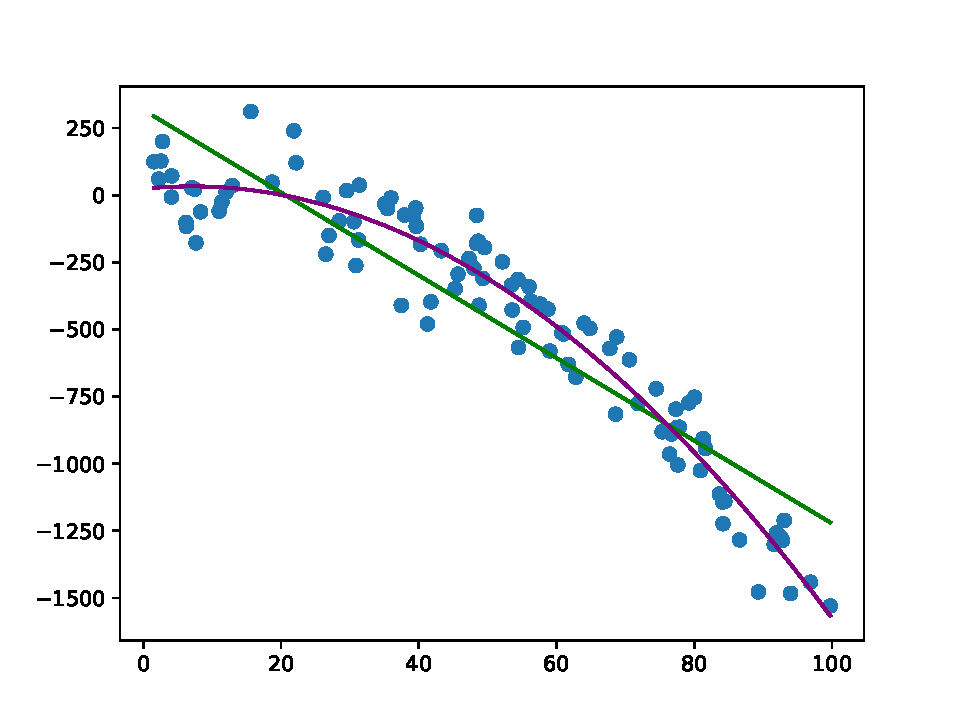
\includegraphics[width=0.8\textwidth]{bestfit.pdf}
\caption{The best-fit line, and best-fit quadratic, to the set of points
generated by the code in Figure~\ref{fig:bestFitCode}.}
\label{fig:bestFitPlot}
\end{figure}


These approximations are called \textbf{parametric} models because they're
based on (global) parameters: a slope and an intercept, say, or three
coefficients in the case of the quadratic. In each case, we assume the data
fit an overall particular ``functional form'' (like a line, or a quadratic) and
say, ``given that we feel like these data are `really' a line, what parameters
that describe a line would give us the best line?''

Figure~\ref{fig:bestFitPlot} shows the best-fit line and best-fit quadratic
(function with an $x^2$ term) for the points generated by the code in
Figure~\ref{fig:bestFitCode}.

\section{LOWESS: a ``non-parametric'' approximation}

A more advanced technique for this task is called ``\textbf{LOWESS}''
(sometimes ``\textbf{LOESS}''\footnote{Some authors make a very fine
distinction between the LOESS and the LOWESS techniques, which is too nitpicky
to even get into here. We'll treat the two terms as synonymous.}), which
(sorta) stands for ``Locally Weighted Estimated Scatterplot Smoothing.''
LOWESS tries to capture the overall trend of a messy set of data -- but what
distinguishes it from a best-fit line is that it operates \textit{locally}
rather than globally. When you crunch the numbers to find the best-fit
least-squares line to a data set, you're asking, ``what values of slope and
intercept for a \textit{single} line across the \textit{entire} data set will
give me the lowest \textit{overall} deviation from the points?'' (The same is
true for a best-fit quadratic, cubic, \textit{etc.}) In other words, you're
attempting to fit a single model over the entire range of data, and penalizing
inaccuracies equally everywhere.

By contrast, the LOWESS technique approximates the data \textit{locally}. This
means that it weights the data points in such a way that points close to the
location of interest contribute more strongly than do data points farther
away. It does this by fitting a linear (or polynomial) regression to each $x$
point of interest, but using a weighted contribution from only the nearby
points.

Here's how it works. We start with a bunch of $(x,y)$ points, and we want to
compute a ``locally smoothed'' $y$ for every one of the $x$'s. 

First, we have a parameter $\alpha$ that specifies \textit{what fraction of
the data} to take into account (at all) for each estimate. This can be any
value from 0 to 1. You might guess that the smaller it is, the more wiggly
it'll allow our smoothed estimate to be, since we'll be considering only a
small number of points. This is true, as we'll see.

Then, once we've fixed $\alpha$, we're going to find a bunch of best-fit,
least-squares lines, one at each $x$ value. This is just like in regular old
linear regression. The catch is that instead of minimizing the \textit{sum} of
squared errors, we're going to minimize the \textbf{weighted} sum. And we'll
place a greater weight on the errors for $x$ points close to the one we're
evaluating. This will have the effect of allowing the curve to bend closely to
our actual data points while ignoring stuff that's far away.

In equations, the best-fit line approach finds an $m$ and $b$ that minimize
the overall sum of squared deviations (or ``residual sum of squares''):

\begin{align*}
RSS = \sum_i (y_i - (mx_i + b))^2
\end{align*}

But with LOWESS, we calculate this separately for every $x$ point, and we
weight this with a \textbf{weight function} $w$:

\begin{align*}
RSS(x) = \sum_i w(x-x_i) \cdot (y_i - (mx_i + b))^2
\end{align*}

Note how the weight function is given the distance between the $x$ value of
interest and the locations of the actual data points. Since we want to weight
close-by points more heavily, the $w$ should be higher for values closer to 
0.\footnote{You might notice that the weight function is much like the
\textit{kernel} for KDEs: in fact, it really is basically a kernel. Thus we
can use a Gaussian for it, just like we did for KDEs, although it's more
common with LOWESS to use the so-called ``tri-cube'' kernel: $w(\Delta x) = (1 -
|\Delta x|^3)^3$ for $|x|<1$ (and 0 otherwise).}

This is \textbf{non-parametric} because when we're done, if somebody asked,
``hey, I like your LOWESS curve -- what parameters did you use for it?'' the
answer would be ``uh...there really aren't any parameters.'' The curve is a
messy combination of a bunch of different shifting approximations that we
calculated as we went through the whole data set. We didn't choose parameters
to plug into a particular model; in fact, we didn't really \textit{have} a
model.

Like KDEs, this technique wasn't computationally possible until the age of
computers. Hence it's one of the newer kids on the block. Here's how to do it
in Python with the \texttt{statsmodel} library:

\begin{Verbatim}[fontsize=\small,samepage=true,frame=single]
import statsmodels.nonparametric.smoothers_lowess

lowess = statsmodels.nonparametric.smoothers_lowess.lowess(y,x,frac=1/3)
plt.plot(lowess[:,0],lowess[:,1],color="red")
\end{Verbatim}

\vspace{.2in}

The ``\texttt{frac}'' parameter is our $\alpha$. The resulting curve for two
different values of $\alpha$ is shown in Figure~\ref{fig:lowess}. Notice how
$\alpha = \frac{1}{3}$ gives a much smoother line than $\alpha =
\frac{1}{10}$, since it is using more points to do the smoothing. In fact, the
former is quite close to the best-fit quadratic in this case. This is a
manifestation of the classic ``bias-variance tradeoff'' we'll talk about later
in the semester.

\begin{figure}[ht]
\centering
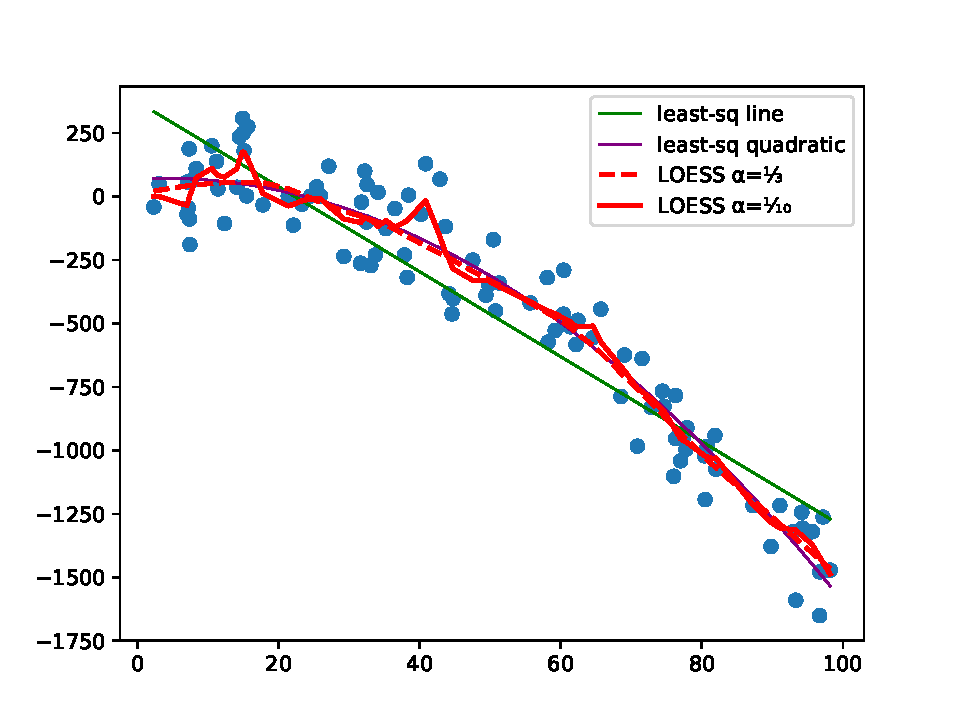
\includegraphics[width=1\textwidth]{lowess.pdf}
\caption{Various attempts to plot the ``true, underlying pattern'' of our
noisy data set.}
\label{fig:lowess}
\end{figure}

LOWESS might not appear to have much of an advantage over just a plain old
line. But Figure~\ref{fig:lowessBetter} shows a data set where neither the
line nor the quadratic are even in the ballpark, but where LOWESS does quite
well. Intuitively, if the data \textit{aren't} ultimately generated by
something linear (or close to it), a linear model will be hard-pressed to
capture the curve.

\begin{figure}[ht]
\centering
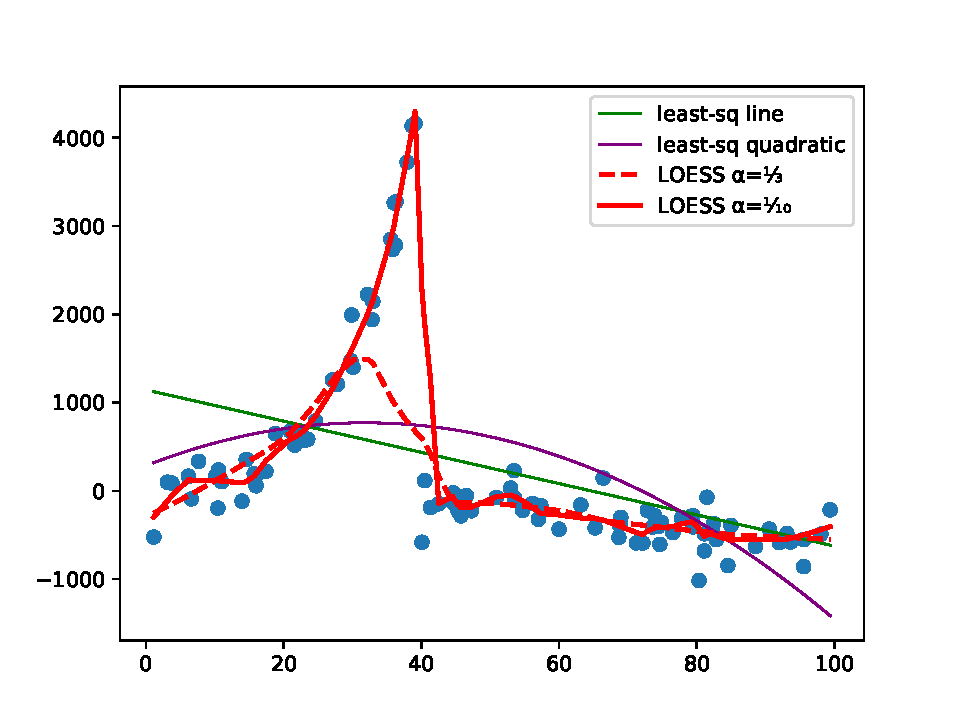
\includegraphics[width=.95\textwidth]{lowess_better.pdf}
\caption{A decidedly non-linear data set, for which LOWESS (and particularly
LOWESS with a low $\alpha$) does quite well.}
\label{fig:lowessBetter}
\end{figure}

In general, LOWESS is a better \textit{exploratory} technique than best-fit
parametric curves are. This is true for a couple of reasons:

\begin{compactitem}

\item When exploring a data set, you're looking for patterns that stick out,
and you want to let the data speak for itself. You're not coming to the data
with a pre-established model choice and wanting to fit it. LOWESS lets you be
model-agnostic and yet see the forest instead of just trees.

\item LOWESS (and non-parametric methods in general) are ``robust,'' meaning
they aren't as adversely affected by outliers. Consider fitting a
least-squares line to a set of data, and then introducing a couple of
high-leverage outliers near one of the far ends. This is going to force your
global-error-minimizing best-fit line to swing radically away from the bulk of
the data (which it may describe fairly adequately) in order to try and reach
those outliers. Clearly this isn't a good fit for the data! LOWESS, however,
will only ``reach'' for those outliers in the $x$ range when it gets near those
outliers.

\end{compactitem}

\vspace{.1in}

By the way, although we fit a \textit{linear} function to each local point, we
could fit a quadratic, cubic, or anything else. Here's something to think
about: if we replaced the linear ``$mx+b$'' function with just a constant
``$b$'', then LOWESS becomes simply a weighted moving average. Oooo, deep.

\vspace{.1in}

Finally, remember to play with the $\alpha$ parameter just as you played with
the kernel width and bin size in other exploratory techniques. Remember:
changing this will give you different views on the data, and different views
are good.


